\documentclass[10pt,a4paper]{article}
\usepackage[utf8]{inputenc}
\usepackage{amsmath}
\usepackage{amsfonts}
\usepackage{amssymb}
\usepackage{graphicx}
\usepackage{hyperref}
\title{Speech Recognition for Low Resource Language-Twi}
\author{\textbf{Lectures:} Gabriel Synnaeve \\ Neil Zeghidour \\ Laurent Besacier \\ Emmanuel Dupoux \\  \textbf{Students:} Yaw Brefo and  Emmanuel Agbeli}
\begin{document}
\maketitle	
\section{Introduction}

In this project, we intend to use pretrained model for our local dialect language known as Twi. This local dialect is one of the dominant speaking languages in Ghana. The goal of the project is to perform speech recognition by using the Constrastive Predicting Coding (CPC) pretrained model and also evaluate the Character Error Rate(CER). 


\section{Challenges}

In this work, we had some few hurdles when undertaking this project. Some of them are: the data collections and computational resources to explore further in different scope of the work. We were limited to using colab platform to compile our analysis without enough GPU. We only had one open-sourced dataset avaliable for the project. 

\section{Data collections}

In the part of our work, we explain the approach used in collecting the dataset. Though the collection was done for individual members of these group but after we had to merge them together in order to split them into train, validation and testing set. The recording was done 2 hours using the holy scripture written in our language, since that was only source of available open-sourced dataset available for this dialect.  In all we had 4 hours of recording where splitted the them into 50$\%$ for both training and testing set respectively and after we took 20 $\%$ of the training set as our validation set for the model. In order to evaluate the performance of the model. 


\section{Materials and methdod}

The Constrastive Predictive Coding (CPC) model was used as pretrained model and fine tune the training set with Connectionist Temporal Classification. This was small Automatic Speech Recognition system for the Twi dialect with their corresponding labeled dataset. 

In the modeling phase, we did character representation of the words in our dialect and also remove all faulty voice recording from each of the folders.  

\section{Results and Discussion}

In the first phase of our analysis, we had to use the CPC model on the dataset without any fine tuning and adding a linear layer as the prediction network. We observe that the average loss for both training and validation are 4.8 and 4.7 respectively. 

\subsection{Fine-tuning results for Character level}

The figure \ref{fig:trainloss} shows the training and validation loss for the character level recognition for the twi language after 50 epochs. This was done by using the pretrained model and also visualize the performance of the model. We observe that, the model outperforms well on the training set than the validation set. 80 $\%$ was use for the training and 20$\%$ for validation. 

\begin{figure}[h]
	\centering
	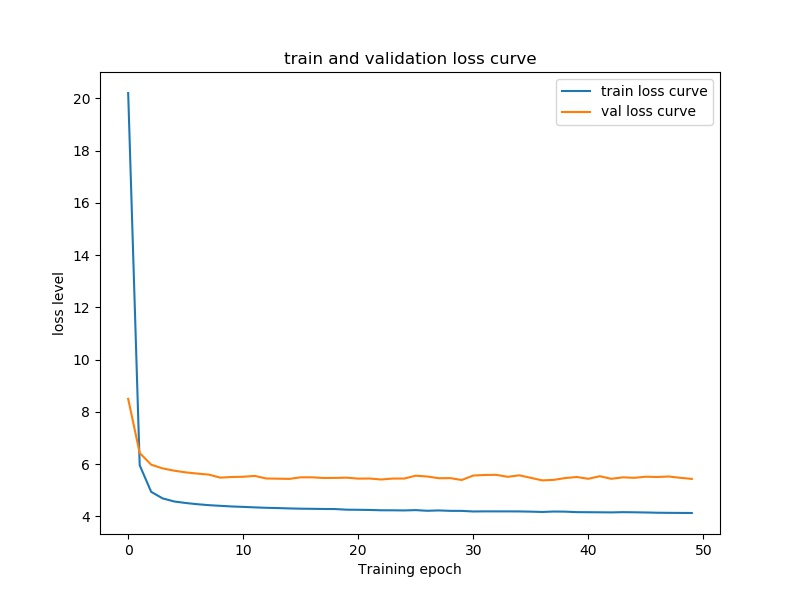
\includegraphics[width=0.6\linewidth]{../train_loss}
	\caption{train and loss curve for character recognition.}
	\label{fig:trainloss}
\end{figure}

On the whole, the average training and validation loss are 4.6 and 5.6 respectively. We realize that there is no wide margin between training and validation loss.  
\begin{table}[h!]
	\begin{center}
		\caption{Summary of CER under fine tuning}
		\label{tab1}
	 \begin{tabular}{|c|c|}
		\hline 
		Evaluation	& CER \\ 
		\hline 
		Validation	& 0.981 \\ 
		\hline  
		Testing &  0.906  \\ \hline
	\end{tabular} 
	\end{center}
\end{table}

The table \ref{tab1} shows a summary of the character error rate for both validation and testing set. The character error rate for the validation is higher compare to the the testing. 

\section{Error Analysis.}

From our perspective, we observe the model perform well on the training set than the validation, which in way we could consider doing overfitting analysis because there is some level oversimplification of data by the model. There should be a tradeoff between bias-variance of the model. 


\section{Further studies}

We intended to explore other pretrained models aside the others we have used on our dataset and also increase the number of recordings and see the how well those models would perform compare to what we have use in our work. 

\subsection{Github links}

Here is the links to our repositories for the source code and dataset. 
\href{https://github.com/YawBrefo/AMMI-2020-Speech-Recognition-Twi-Audio-dataset}{Yaw}  and 
 \href{https://github.com/Agbeli/Speech_recognition_AMMI}{Emmanuel}. Click on the names to have access to individual repository. 









\end{document}